% Options for packages loaded elsewhere
\PassOptionsToPackage{unicode}{hyperref}
\PassOptionsToPackage{hyphens}{url}
\PassOptionsToPackage{dvipsnames,svgnames*,x11names*}{xcolor}
%
\documentclass[
  openany]{book}
\usepackage{lmodern}
\usepackage{amssymb,amsmath}
\usepackage{ifxetex,ifluatex}
\ifnum 0\ifxetex 1\fi\ifluatex 1\fi=0 % if pdftex
  \usepackage[T1]{fontenc}
  \usepackage[utf8]{inputenc}
  \usepackage{textcomp} % provide euro and other symbols
\else % if luatex or xetex
  \usepackage{unicode-math}
  \defaultfontfeatures{Scale=MatchLowercase}
  \defaultfontfeatures[\rmfamily]{Ligatures=TeX,Scale=1}
\fi
% Use upquote if available, for straight quotes in verbatim environments
\IfFileExists{upquote.sty}{\usepackage{upquote}}{}
\IfFileExists{microtype.sty}{% use microtype if available
  \usepackage[]{microtype}
  \UseMicrotypeSet[protrusion]{basicmath} % disable protrusion for tt fonts
}{}
\makeatletter
\@ifundefined{KOMAClassName}{% if non-KOMA class
  \IfFileExists{parskip.sty}{%
    \usepackage{parskip}
  }{% else
    \setlength{\parindent}{0pt}
    \setlength{\parskip}{6pt plus 2pt minus 1pt}}
}{% if KOMA class
  \KOMAoptions{parskip=half}}
\makeatother
\usepackage{xcolor}
\IfFileExists{xurl.sty}{\usepackage{xurl}}{} % add URL line breaks if available
\IfFileExists{bookmark.sty}{\usepackage{bookmark}}{\usepackage{hyperref}}
\hypersetup{
  pdftitle={ MT3508: Applied Statistics (2020/2021)},
  colorlinks=true,
  linkcolor=Maroon,
  filecolor=Maroon,
  citecolor=Blue,
  urlcolor=Blue,
  pdfcreator={LaTeX via pandoc}}
\urlstyle{same} % disable monospaced font for URLs
\usepackage{longtable,booktabs}
% Correct order of tables after \paragraph or \subparagraph
\usepackage{etoolbox}
\makeatletter
\patchcmd\longtable{\par}{\if@noskipsec\mbox{}\fi\par}{}{}
\makeatother
% Allow footnotes in longtable head/foot
\IfFileExists{footnotehyper.sty}{\usepackage{footnotehyper}}{\usepackage{footnote}}
\makesavenoteenv{longtable}
\usepackage{graphicx,grffile}
\makeatletter
\def\maxwidth{\ifdim\Gin@nat@width>\linewidth\linewidth\else\Gin@nat@width\fi}
\def\maxheight{\ifdim\Gin@nat@height>\textheight\textheight\else\Gin@nat@height\fi}
\makeatother
% Scale images if necessary, so that they will not overflow the page
% margins by default, and it is still possible to overwrite the defaults
% using explicit options in \includegraphics[width, height, ...]{}
\setkeys{Gin}{width=\maxwidth,height=\maxheight,keepaspectratio}
% Set default figure placement to htbp
\makeatletter
\def\fps@figure{htbp}
\makeatother
\setlength{\emergencystretch}{3em} % prevent overfull lines
\providecommand{\tightlist}{%
  \setlength{\itemsep}{0pt}\setlength{\parskip}{0pt}}
\setcounter{secnumdepth}{5}
\usepackage{booktabs}
\usepackage{longtable}
\usepackage{amsthm}
\usepackage{amsmath}

\makeatletter
\def\thm@space@setup{%
  \thm@preskip=8pt plus 2pt minus 4pt
  \thm@postskip=\thm@preskip
}
\makeatother

\usepackage{makeidx}
%\makeindex

\ifxetex
  \usepackage{letltxmacro}
  \setlength{\XeTeXLinkMargin}{1pt}
  \LetLtxMacro\SavedIncludeGraphics\includegraphics
  \def\includegraphics#1#{% #1 catches optional stuff (star/opt. arg.)
    \IncludeGraphicsAux{#1}%
  }%
  \newcommand*{\IncludeGraphicsAux}[2]{%
    \XeTeXLinkBox{%
      \SavedIncludeGraphics#1{#2}%
    }%
  }%
\fi

% ~~~~~~~~~~~~~~~~~~~~~~~~~~~~~~~~~~~~~~~~~~~~~~
% ~~~~~~~~~~~~~~~~~~~~~~~~~~~~~~~~~~~~~~~~~~~~~~





% latex macro to create task boxes
\usepackage{tcolorbox}
\tcbuselibrary{breakable}

\definecolor{taskCol}{HTML}{00539b}
\definecolor{taskCol1}{HTML}{007870}

\tcbset{colback=white,colframe=taskCol,arc=0mm}

%trick to fool markdown into compiling
\newcommand{\bblockT}[2][Task]{\begin{tcolorbox}[title = #1 #2, parbox = false]}
\newcommand{\eblockT}{\end{tcolorbox}}
\newcommand{\bblockS}[2][Solution]{\begin{tcolorbox}[title = #1 #2, colframe=taskCol1, breakable, parbox = false]}
\newcommand{\eblockS}{\end{tcolorbox}}

%add tabbed solutions environment
\newcommand{\bmp}{\begin{minipage}[c]{0.5\textwidth}}
\newcommand{\emp}{\end{minipage}}
\newcommand{\bblockST}[1]{\begin{tcolorbox}[title = #1, colframe=taskCol1, breakable, parbox = false]}
\newcommand{\eblockST}{\end{tcolorbox}}

%set solution button link
\usepackage{tikz}

\newcommand{\buttonT}[1]{
    \begin{tikzpicture}
    \node[
        inner sep=5pt,
        draw=taskCol,
        fill=taskCol,
        rounded corners=2pt,
        text=white
    ] (c1) {#1};
    \end{tikzpicture}
}

\newcommand{\buttonS}[1]{
    \begin{tikzpicture}
    \node[
        inner sep=5pt,
        draw=taskCol1,
        fill=taskCol1,
        rounded corners=2pt,
        text=white
    ] (c1) {#1};
    \end{tikzpicture}
}

\newcommand{\colpageref}[1]{\hypersetup{linkcolor=white}\pageref{#1}}
\usepackage[]{natbib}
\bibliographystyle{apalike}

\title{
\includegraphics[width=1in,height=\textheight]{standard-vertical-black.png} MT3508: Applied Statistics (2020/2021)}
\author{}
\date{\vspace{-2.5em}26 January 2021}

\begin{document}
\maketitle

{
\hypersetup{linkcolor=}
\setcounter{tocdepth}{1}
\tableofcontents
}
\hypertarget{contact-information}{%
\chapter*{Contact Information}\label{contact-information}}
\addcontentsline{toc}{chapter}{Contact Information}

\textbf{\emph{Important: Please check \href{https://moody.st-andrews.ac.uk/moodle/}{Moodle} and Teams regularly for announcements.}}

\textbf{Module Co-ordinator:} Dr Hannah Worthington

\textbf{Lecturers:} Dr Hannah Worthington and Dr Michail Papathomas

\textbf{Contact Information:}

Please use email or Teams to contact us.

\begin{itemize}
\tightlist
\item
  Hannah: \href{mailto:hw233@st-andrews.ac.uk}{hw233@}
\item
  Michail: \href{mailto:M.Papathomas@st-andrews.ac.uk}{M.Papathomas@}
\end{itemize}

Please begin the email subject with \emph{MT3508}.

\hypertarget{module-description}{%
\chapter*{Module Description}\label{module-description}}
\addcontentsline{toc}{chapter}{Module Description}

Together with MT3507, this module provides a bridge between second year and Honours modules in Statistics. It deals with the application of statistical methods to test hypotheses and draw inferences from data. This includes a number of nonparametric methods and statistical tests (goodness-of-fit tests and tests of independence). Inference methods include model fitting by least squares and maximum likelihood, and variance estimation by means of the information matrix and the bootstrap. The framework of the generalised linear model is presented covering parameter estimation, deviance, model selection and diagnostics. Further applications include multiple regression, analysis of variance and the (normal) linear model.

\textbf{\emph{Pre-requisites}}: Before taking this module you must pass MT2508.

\hypertarget{intended-learning-outcomes}{%
\section*{Intended Learning Outcomes}\label{intended-learning-outcomes}}
\addcontentsline{toc}{section}{Intended Learning Outcomes}

\begin{itemize}
\item
  Understand inference by maximum likelihood sufficiently well to conduct maximum likelihood inference on unseen problems using the statistical software \texttt{R}, and to draw appropriate conclusions.
\item
  Be able to construct appropriate likelihood functions from non-mathematical problem descriptions, for problems involving uncertainty, and in which observations are independent.
\item
  Be able to use \texttt{R} to implement likelihood functions, to maximise them with respect to unknown parameters, and obtain confidence intervals for model parameters and functions of parameters.
\item
  Understand the relationships between ANOVA models, linear regression models, generalised linear models, and more general statistical models that do not fall into any of these categories.
\item
  Be able to conduct appropriate model selection and diagnostic tests for these models, to assess model adequacy.
\item
  Be able to obtain Wald confidence intervals, profile likelihood confidence intervals, and bootstrap confidence intervals for parameters and functions of parameters.
\end{itemize}

\hypertarget{timetable}{%
\chapter*{Timetable}\label{timetable}}
\addcontentsline{toc}{chapter}{Timetable}

The following information may change as the semester develops. Whilst I shall endeavour to keep this document up-to-date, please regularly check Moodle and Teams for announcements of any changes. Get in touch if anything is unclear.

I'll introduce the module during a live Teams session on \textbf{\emph{Tuesday 26th January 12pm (Week 1)}}. Come along with suggestions or questions about the semester.

\hypertarget{lectures}{%
\section*{Lectures}\label{lectures}}
\addcontentsline{toc}{section}{Lectures}

Lectures will take place over Teams on Mondays (even weeks only), Tuesdays and Thursday at 12pm Noon. The sessions will be recorded and available through the module \href{https://moody.st-andrews.ac.uk/moodle/}{Moodle page} (hopefully later the same day).

Below is a \emph{rough} schedule indicating which parts of the lecture notes are to be covered each week. Please see the \textbf{\emph{Lecture Plan}} document for information on individual sessions.

\begin{itemize}
\tightlist
\item
  \textbf{\emph{Week 1}} - Introduction to the module and \emph{Section 1.1} introducing some examples that will carry through the module
\item
  \textbf{\emph{Week 2}} - Finish \emph{Chapter 1} and start \emph{Chapter 2} up to discussing \texttt{optim}
\item
  \textbf{\emph{Week 3}} - Finish \emph{Chapter 2}
\item
  \textbf{\emph{Week 4}} - \emph{Chapter 3} and start \emph{Chapter 4} up to beginning to discuss goodness-of-fit tests
\item
  \textbf{\emph{Week 5}} - Finish \emph{Chapter 4}
\item
  \textbf{\emph{Week 6}} - \emph{Chapter 5} up to starting to look at examples
\item
  \textbf{\emph{Week 7}} - Finish \emph{Chapter 5} and start \emph{Chapter 6} up to beginning to look at one-way ANOVA
\item
  \textbf{\emph{Week 8}} - \emph{Chapter 6} possibly finish two-way ANOVA
\end{itemize}

\textbf{Spring Break}

\begin{itemize}
\tightlist
\item
  \textbf{\emph{Week 9}} - \emph{Chapter 6} regression, looking at examples and diagnostics
\item
  \textbf{\emph{Week 10/11}} - Finish \emph{Chapter 6}
\end{itemize}

\hypertarget{practical-sessions}{%
\section*{Practical Sessions}\label{practical-sessions}}
\addcontentsline{toc}{section}{Practical Sessions}

This module is very hands-on in using \texttt{R}. Starting in Week 2 there will be weekly practical sessions during which you can discuss and get help on the question sheets.

Practical sessions will take place over Teams and we will be using R-Studio Cloud as a means to share code. We'd like to make use of the breakout rooms in teams to see some small group discussions taking place amongst the class, so please do your best to attend a session each week.

For Weeks 2-11 the weekly sessions will take place on:

\textbf{\emph{Thursday 10am and Thursday 3pm}}

You'll be able to sign up for a group on MySaint, but you are welcome to attend both if you wish!

\hypertarget{office-hours}{%
\section*{Office Hours}\label{office-hours}}
\addcontentsline{toc}{section}{Office Hours}

If you have questions about the module materials you are welcome to get in touch over email or Teams at any point. If you have queries you want to discuss in real time (i.e.~live face-to-face over teams) then you can make use of the following office hour:

\textbf{\emph{Wednesday 12pm Weeks 1-11}}.

\hypertarget{assessment}{%
\chapter*{Assessment}\label{assessment}}
\addcontentsline{toc}{chapter}{Assessment}

\hypertarget{moodle-quizzes---4-times-5}{Moodle Quizzes - 4 \textbackslash times 5\%}}\label{moodle-quizzes---4-times-5}}
\addcontentsline{toc}{subsubsection}{Moodle Quizzes - 4 \(\times\) 5\%}

\textbf{Quiz 1:} Due \textbf{\emph{Wednesday February 10th 1pm (Week 3)}}

\textbf{Quiz 2:} Due \textbf{\emph{Wednesday February 24th 1pm (Week 5)}}

\textbf{Quiz 3:} Due \textbf{\emph{Wednesday March 17th 1pm (Week 8)}}

\textbf{Quiz 4:} Due \textbf{\emph{Wednesday April 14th 1pm (Week 10)}}

There will also be a practice quiz in Week 2 so that you can see the potential format and some of the different styles of questions that may be asked.

\hypertarget{final-exam---80}\label{final-exam---80}}
\addcontentsline{toc}{subsubsection}{Final Exam - 80\%}

You must complete at least 90\% of assessment in a module to have the opportunity to gain credit in the module. If you do not complete at least 90\% of assessment you will be given a FINAL academic alert in the module and receive a grade of 0X.

\hypertarget{r-studio-cloud}{%
\chapter*{R-Studio Cloud}\label{r-studio-cloud}}
\addcontentsline{toc}{chapter}{R-Studio Cloud}

\textbf{\emph{Warning}}: I'm also rather new to using R-Studio Cloud. (In fact some of you may have already logged more hours if you have met it in other modules\ldots) So this is a learning experience for everyone.

\hypertarget{what-is-r-studio-cloud}{%
\section*{What is R-Studio Cloud?}\label{what-is-r-studio-cloud}}
\addcontentsline{toc}{section}{What is R-Studio Cloud?}

This is a version of R-Studio that runs in your browser as a cloud-based solution for remote collaboration, code sharing and teaching.

You can access R-Studio Cloud \href{https://login.rstudio.cloud/login?setup=1\&redirect=\%2Foauth\%2Fauthorize\%3Fresponse_type\%3Dcode\%26client_id\%3Drstudio-cloud\%26show_auth\%3D0\%26redirect_uri\%3Dhttps\%253A\%252F\%252Frstudio.cloud\%252Flogin\%26show_login\%3D1}{here}. When you enter your university email address an option will appear to allow you to log-in through the University. Access is still being arranged so some of you may not be able to do so just yet, but it should be possible very shortly.

\hypertarget{why-are-we-using-r-studio-cloud}{%
\section*{Why are we using R-Studio Cloud?}\label{why-are-we-using-r-studio-cloud}}
\addcontentsline{toc}{section}{Why are we using R-Studio Cloud?}

You will be getting a fair bit of programming practice in this module. Ordinarily we would be teaching in an environment where tutors can simply look over your shoulder to help out or offer suggestions.

This is rather tricky at the moment.

If/when issues arise, the most efficient way to offer help is to be able to see \textbf{\emph{exactly}} the problems you are having.

It's my experience that screen sharing/emailing code/screen grab/copying the error message, only offers a quick fix when the issue is trivial. It is a frequent problem that the errors can not be recreated or there are version issues/updates/missing packages/missing information/other conflicts that cause more problems.

R-Studio Cloud gets around this by allowing tutors to see your work exactly as you are seeing it, error messages and all. We hope (and we are taking a bit of a leap of faith here) that the R-Studio Cloud is a straightforward way to offer help on coding in a way that is efficient, but still familiar, for everyone involved.

\hypertarget{how-will-we-use-r-studio-cloud}{%
\section*{How will we use R-Studio Cloud?}\label{how-will-we-use-r-studio-cloud}}
\addcontentsline{toc}{section}{How will we use R-Studio Cloud?}

Each practical sheet will have it's own project area in R-Studio Cloud. These are projects that I will create and then share with you, from which you can duplicate a copy and then work on just as you would in R-Studio normally.

The idea is, if you run into problems you can let a tutor know and they can jump into your session to see what is happening.

\textbf{\emph{Pros:}}

\begin{itemize}
\tightlist
\item
  You can continue working on your code whilst waiting for help.
\item
  When a tutor takes a look they are seeing the most up-to-date version.
\item
  The tutor can see all of your code. This is particularly helpful since error messages are often associated with something earlier on going astray and only being flagged later on.
\item
  You can work asynchronously to the tutor but only have one version on the go.
\item
  It avoids AppsAnywhere!
\end{itemize}

\textbf{\emph{Cons:}}

\begin{itemize}
\tightlist
\item
  The system isn't perfect. You will temporarily lose access to your work whilst a tutor is taking a look. If you see the following pop-up
\end{itemize}

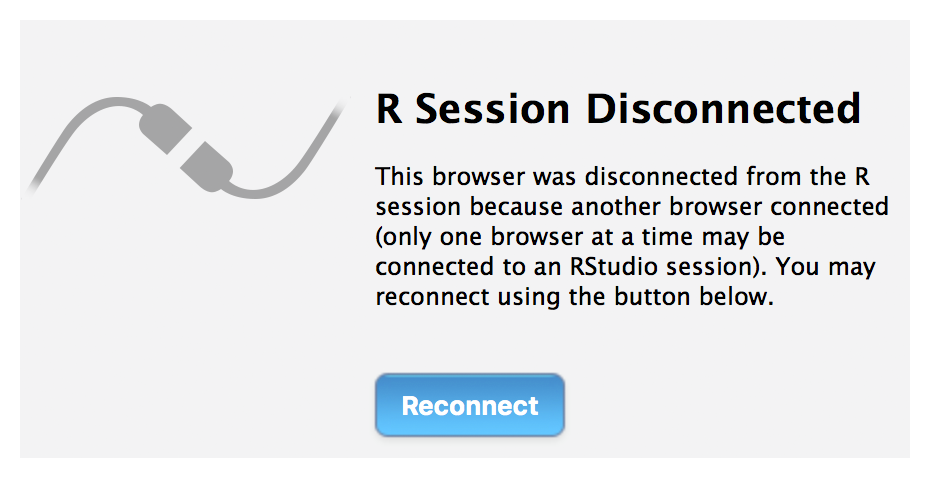
\includegraphics{Figures/disconnected.png}

it's probably an indication that a tutor has jumped into your area and is taking a look at your work.

\begin{itemize}
\tightlist
\item
  We will need to figure out a workflow for requesting help etc.
\item
  You will lose access when term ends (I don't know the exact date).
\end{itemize}

At any point you can download a copy of your work. I will send out reminders to do so as we complete the practical sheets so that you can retain copies of your work.

\hypertarget{what-about-r-studio-desktop}{%
\section*{What about R-Studio desktop}\label{what-about-r-studio-desktop}}
\addcontentsline{toc}{section}{What about R-Studio desktop}

If you would prefer to work on your local version of R-Studio, offline, then you are welcome to do so. But R-Studio Cloud will be the mechanism through which we will be offering coding and teaching support (so you may just need to move your work round a little).

\hypertarget{reference-books}{%
\chapter*{Reference Books}\label{reference-books}}
\addcontentsline{toc}{chapter}{Reference Books}

There is no single text that covers everything that we will do in MT3508. The notes and practicals are comprehensive for our purposes. However, if you would like some supplementary reading, the following books cover various bits of the module.

\hypertarget{ebooks}{%
\section*{eBooks}\label{ebooks}}
\addcontentsline{toc}{section}{eBooks}

The following are available as eBooks through the library.

\href{https://encore.st-andrews.ac.uk/iii/encore/record/C__Rb2496019__SGeneralized\%20additive\%20models\%3A\%20An\%20introduction\%20with\%20R__Orightresult__U__X4?lang=eng\&suite=def}{\textbf{Wood, S. N. (2017). \emph{Generalized additive models: An introduction with R (2nd edition)}. CRC Press}}

While we do not cover generalised additive models (GAMs) in MT3508, this book contains a lot of stuff that we do cover in its lead-up to GAMs.

\begin{itemize}
\tightlist
\item
  Appendix A contains some general maximum likelihood results.
\item
  Chapter 3 contains a lot of good material on GLMs - treated with more theoretical rigour than we do in MT3508, but also some examples of applications of GLMs using R.
\item
  Chapter 1 contains a lot of good material on linear models (LMs: linear regression and ANOVA) - again treated with more theoretical rigour than we do in MT3508, but also some examples of applications of LMs.
\end{itemize}

\href{https://encore.st-andrews.ac.uk/iii/encore/record/C__Rb3040989__SCore\%20statistics__Orightresult__U__X7?lang=eng\&suite=def}{\textbf{Wood, S. N. (2015). \emph{Core statistics}. Cambridge University Press.}}

This is an excellend reference text at a fairly advanced level. The Preface says \emph{``The aim is to offer a concise coverage of the core knowledge needed to understand and use parametric statistical methods and to build new methods for analysing data.''} It does this very well, but much of its contents is beyond the scope of MT3508. The most useful chapter to use are probably:

\begin{itemize}
\tightlist
\item
  Chapter 3, which covers basic R programming and concepts;
\item
  Chapter 4, which covers maximum likelihood theory (often at a more advanced level than MT3508 does); and
\item
  Chapter 7, which covers LMs (often at a more advanced level than MT3508 does).
\end{itemize}

\hypertarget{print}{%
\section*{Print}\label{print}}
\addcontentsline{toc}{section}{Print}

The following is \emph{not} available as an eBook but you may be able to request a scan of appropriate sections from the library.

\href{https://encore.st-andrews.ac.uk/iii/encore/record/C__Rb1908113__SMaximum\%20likelihood\%20estimation\%20and\%20inference\%2C\%20with\%20examples\%20in\%20R\%2C\%20SAS\%20and\%20ADMB__Orightresult__U__X4?lang=eng\&suite=def}{\textbf{Miller, R. B. (2011). \emph{Maximum likelihood estimation and inference, with examples in R, SAS and ADMB}. Wiley}}

This covers a lot more than we do, and is more advanced in many places.

\begin{itemize}
\tightlist
\item
  Chapters 1-6 overlap a good deal with what we do in MT3508.
\item
  The first part of Chapter 7 covers some material on generalised linear models (GLMs).
\item
  Chapters 11 and 12 cover the theory underlying maximum likelihood methods (some of which we use explicitly in MT3508 but none of which we derive; these Chapters contain derivations).
\end{itemize}

  \bibliography{book.bib,packages.bib}

\printindex

\end{document}
